
\chapter{Implementacija i korisničko sučelje}
		
		
		\section{Korištene tehnologije i alati}
		
		%\textbf{\textit{dio 2. revizije}}
			
			 %\textit{Detaljno navesti sve tehnologije i alate koji su primijenjeni pri izradi dokumentacije i aplikacije. Ukratko ih opisati, te navesti njihovo značenje i mjesto primjene. Za svaki navedeni alat i tehnologiju je potrebno \textbf{navesti internet poveznicu} gdje se mogu preuzeti ili više saznati o njima}.
            Komunikacija u timu ostvarena je korištenjem aplikacija \underline{\href{https://web.whatsapp.com/}{WhatsApp}} i \underline{\href{https://discord.com/}{Discord}}, za izradu UML dijagrama korišten je alat \underline{\href{https://astah.net/}{Astah UML}}, a za organizaciju i upravljanje izvornim kodom korišten je sustav \underline{\href{https://git-scm.com/}{Git}}. Kao udaljeni repozitorij projekta korištena je web platforma \underline{\href{https://gitlab.com/}{GitLab}}. Za oblikovanje dokumentacije korišten je alat \underline{\href{www.overleaf.com}{Overleaf}} koji omogućuje prevođenje jezika LaTeX bez posebnih alata.
            \\
            \\
            Razvojno okruženje korišteno za izradu \textit{backend} dijela aplikacije je \underline{\href{https://www.jetbrains.com/idea/}{Jetbrains IntelliJ IDEA}}, IntelliJ olakšava razvoj aplikacija i web-stranica u programskom jeziku Java (uz Spring boot). Za izradu \textit{frontend} dijela aplikacije korišten je \underline{\href{https://code.visualstudio.com/}{Visual Studio Code}} razvojno okruženje s obzirom da treba koristiti više tehnologija odjednom: React, Javascript, Typescript, CSS i slično.
            Za bazu podataka korišten je PostgreSQL a za upravljanje bazom podataka korišten je alat \underline{\href{https://dbeaver.io/}{DBeaver}}.
			
			
			\eject 
		
	
		\section{Ispitivanje programskog rješenja}
			
			\subsection{Ispitivanje komponenti}
			Provedeno je ispitivanje komponenti koristeći okvire za jedinično ispitivanje \underline{\href{https://junit.org/junit5/}{JUnit}} i \underline{\href{https://site.mockito.org/}{Mockito}}. 
           \\
           \\
           Ispituju se metode razreda \textit{BadgeService}, \textit{LocationService} te \textit{TripService}. Ispitni slučajevi sadrže ispitivanje regularnog ponašanja te bacanja iznimki. 
           \\
           \\
           Prije pokretanja ispitnih slučajeva inicijaliziraju se objekti korišteni u ispitnim slučajevima u \textit{initData()} metodi koja je anotirana s \textit{@BeforeEach} (zbog njene duljine, navedena metoda nije prikazana na slikama).
			
        \begin{figure}[H]
            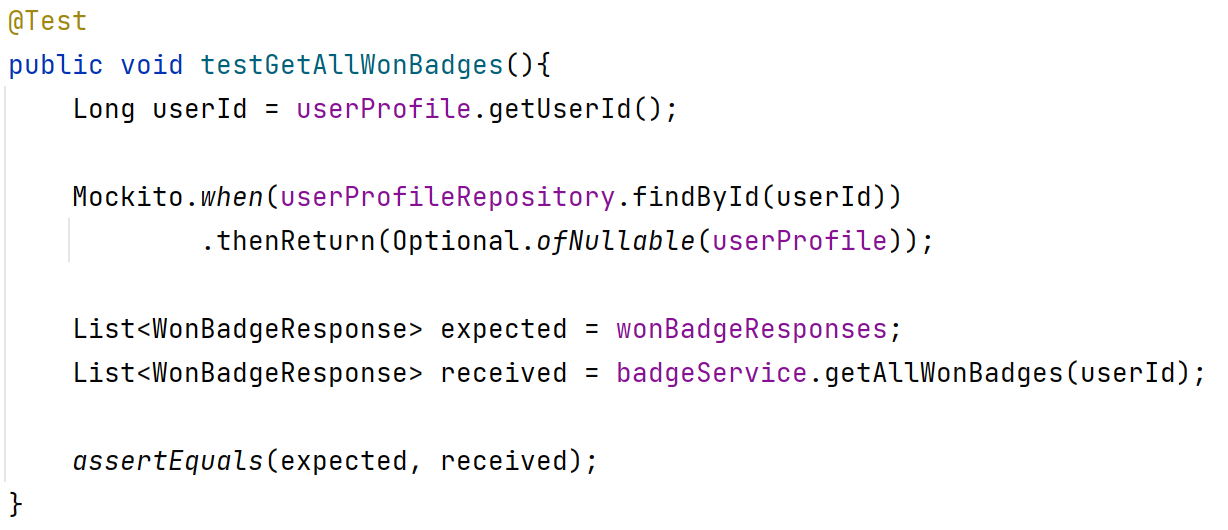
\includegraphics[scale=0.9]{slike/unit_test_badge_get_all.png} 
              \centering
            \caption{Ispitni slučaj - razred \textit{BadgeService} - metoda \textit{getAllWonBadges}}
        \end{figure}

         \begin{figure}[H]
            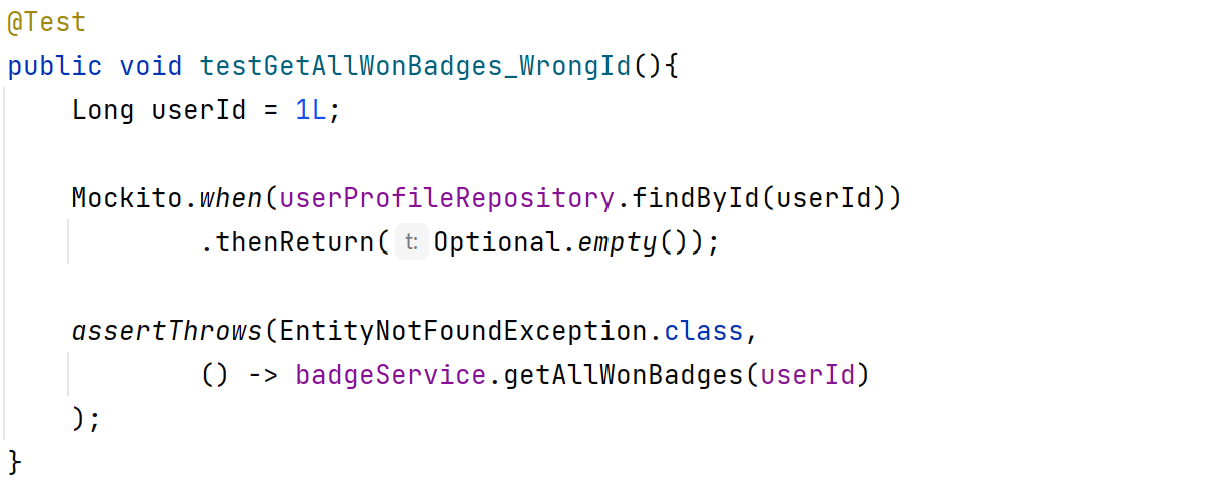
\includegraphics[scale=0.9]{slike/unit_test_location_wrong_id.png} 
              \centering
            \caption{Ispitni slučaj - razred \textit{BadgeService} - metoda \textit{getAllWonBadges} - bacanje iznimke}
        \end{figure}

        \begin{figure}[H]
            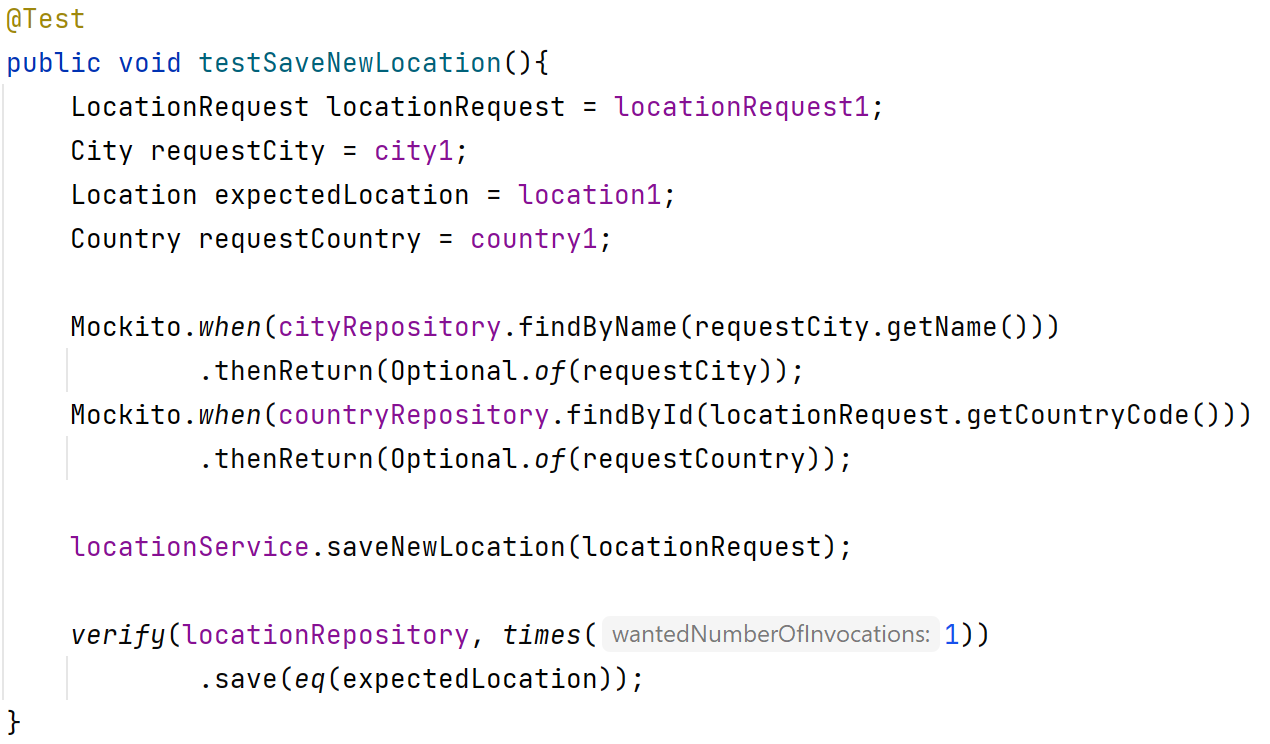
\includegraphics[scale=0.9]{slike/unit_test_location_save.png} 
              \centering
            \caption{Ispitni slučaj - razred \textit{LocationService} - metoda \textit{saveNewLocation}}
        \end{figure}

        \begin{figure}[H]
            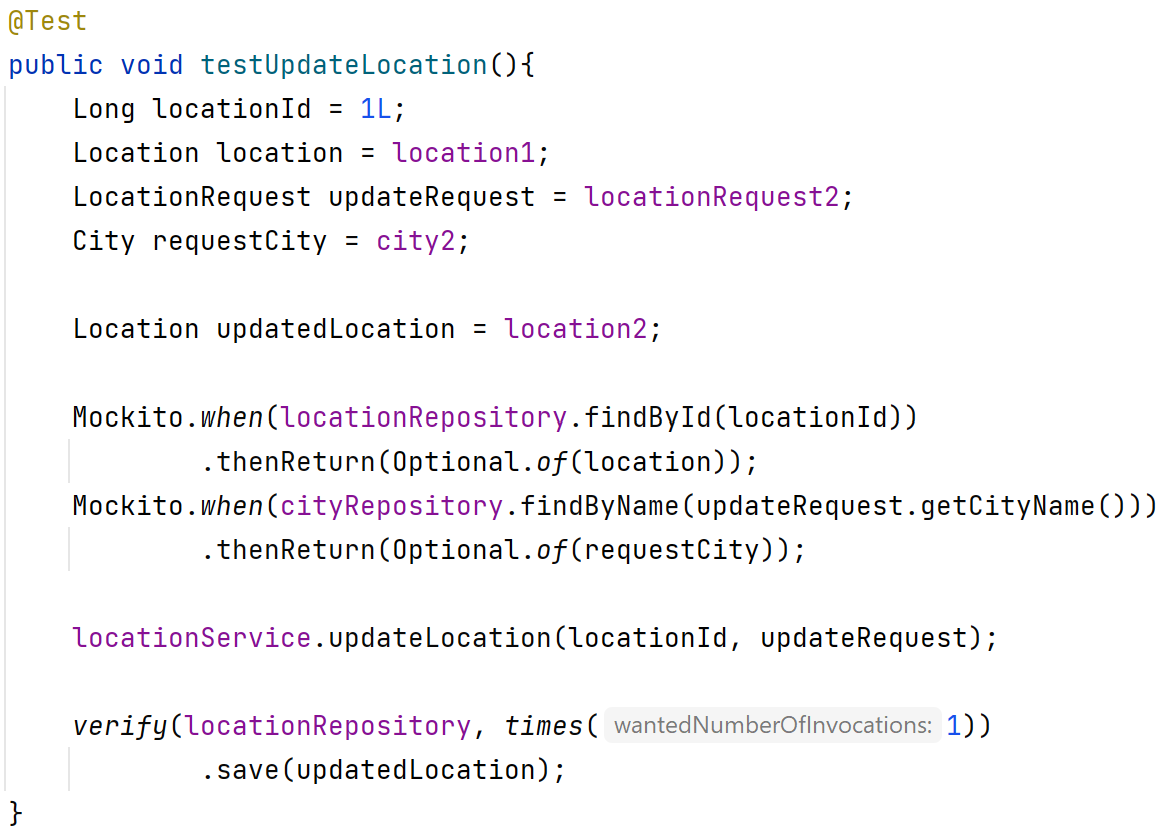
\includegraphics[scale=0.9]{slike/unit_test_location_update.png} 
              \centering
            \caption{Ispitni slučaj - razred \textit{BadgeService} - metoda \textit{updateLocation}}
        \end{figure}

        \begin{figure}[H]
            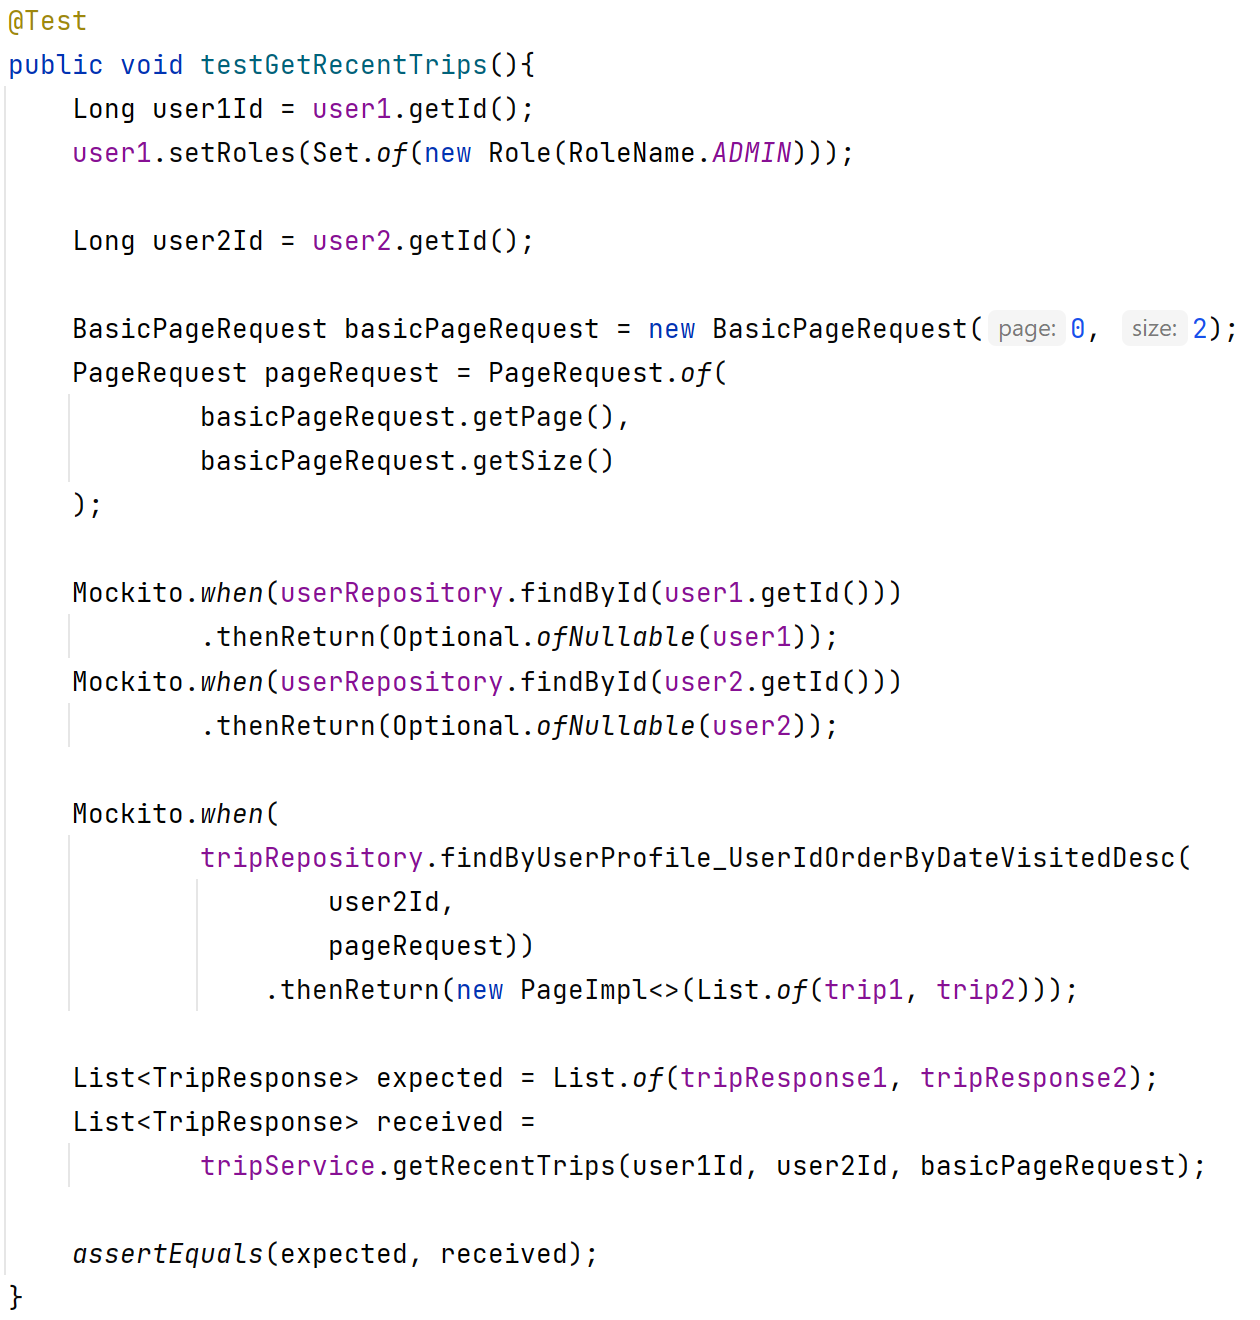
\includegraphics[scale=0.9]{slike/unit_test_trip_recent.png} 
              \centering
            \caption{Ispitni slučaj - razred \textit{TripService} - metoda \textit{getAllWonBadges} - bacanje iznimke}
        \end{figure}

        \begin{figure}[H]
            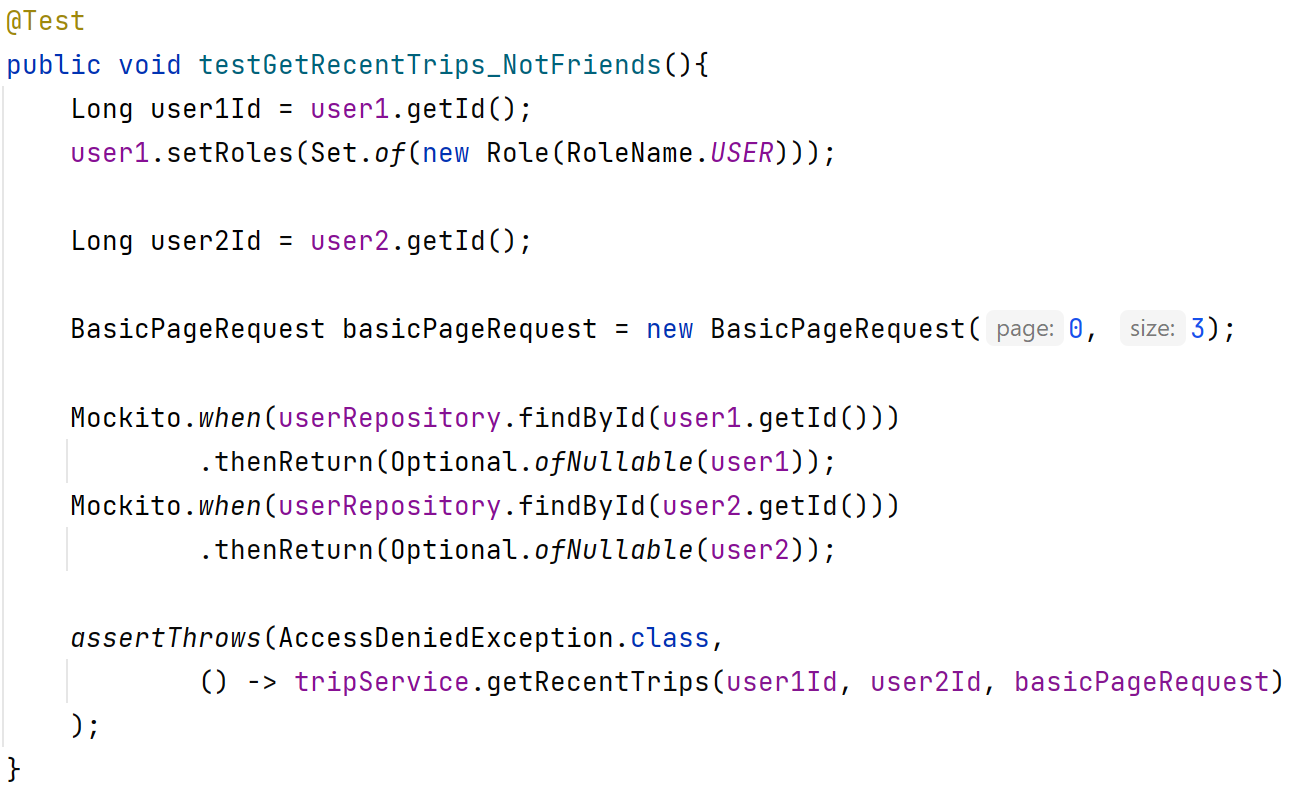
\includegraphics[scale=0.9]{slike/unit_test_trip_not_friends.png} 
              \centering
            \caption{Ispitni slučaj - razred \textit{TripService} - metoda \textit{getRecentTrips} - bacanje iznimke}
        \end{figure}

        \begin{figure}[H]
            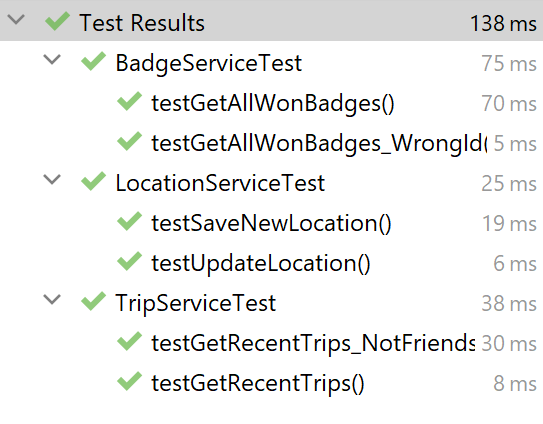
\includegraphics[scale=1]{slike/unit_test_results.png} 
              \centering
            \caption{Rezultati ispitivanja komponenti}
        \end{figure}
        \eject
        
			
			\subsection{Ispitivanje sustava}
			
			 Provedeno je ispitivanje sustava koristeći \underline{\href{https://www.selenium.dev/}{Selenium WebDriver}} (uz Chrome-ov WebDriver) u programskom jeziku Java uz pomoć okvira za jedinično ispitivanje \underline{\href{https://junit.org/junit5/}{JUnit}}. 
            \\
            \\
            Konstante koje završavaju na \textit{XPATH} predstavljaju izravnu putanju do elementa na stranici. Konstanta \textit{{BASE\_URL}} predstavlja URL web stranice. Prije pokretanja testova pokreće se funkcija \textit{initDriver()} koja inicijalizira WebDriver. 
            \\
            \\
            Kako bi se uspješno izvršili ispitni slučajevi u sustavu mora postojati registrirani korisnik s korisničkim imenom "\textit{user}" te lozinkom "\textit{password123}" te ne smije postojati korisnik s korisničkim imenom "\textit{NameSurname}".

                \begin{figure}[H]
        		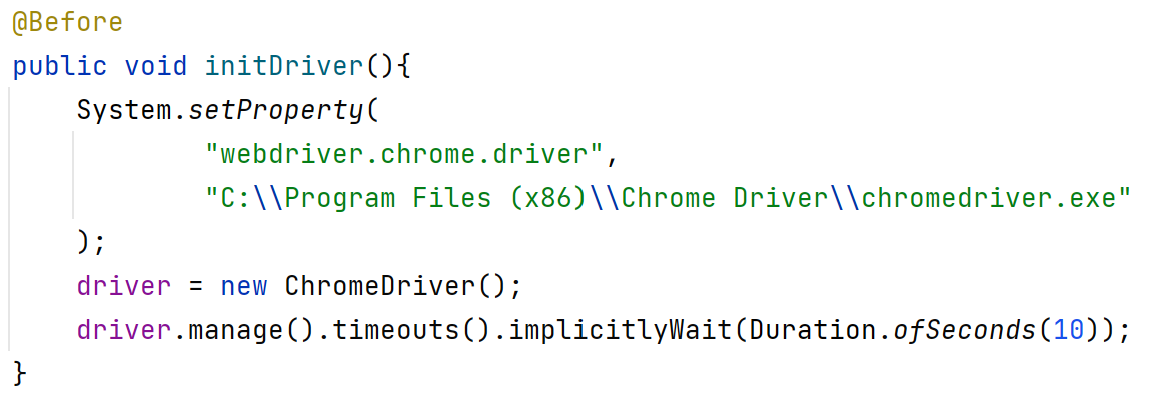
\includegraphics[scale=1]{slike/integration_test_init.png} 
        		  \centering
        		\caption{Inicijalizacija WebDriver-a}
        	\end{figure}

                \begin{figure}[H]
        		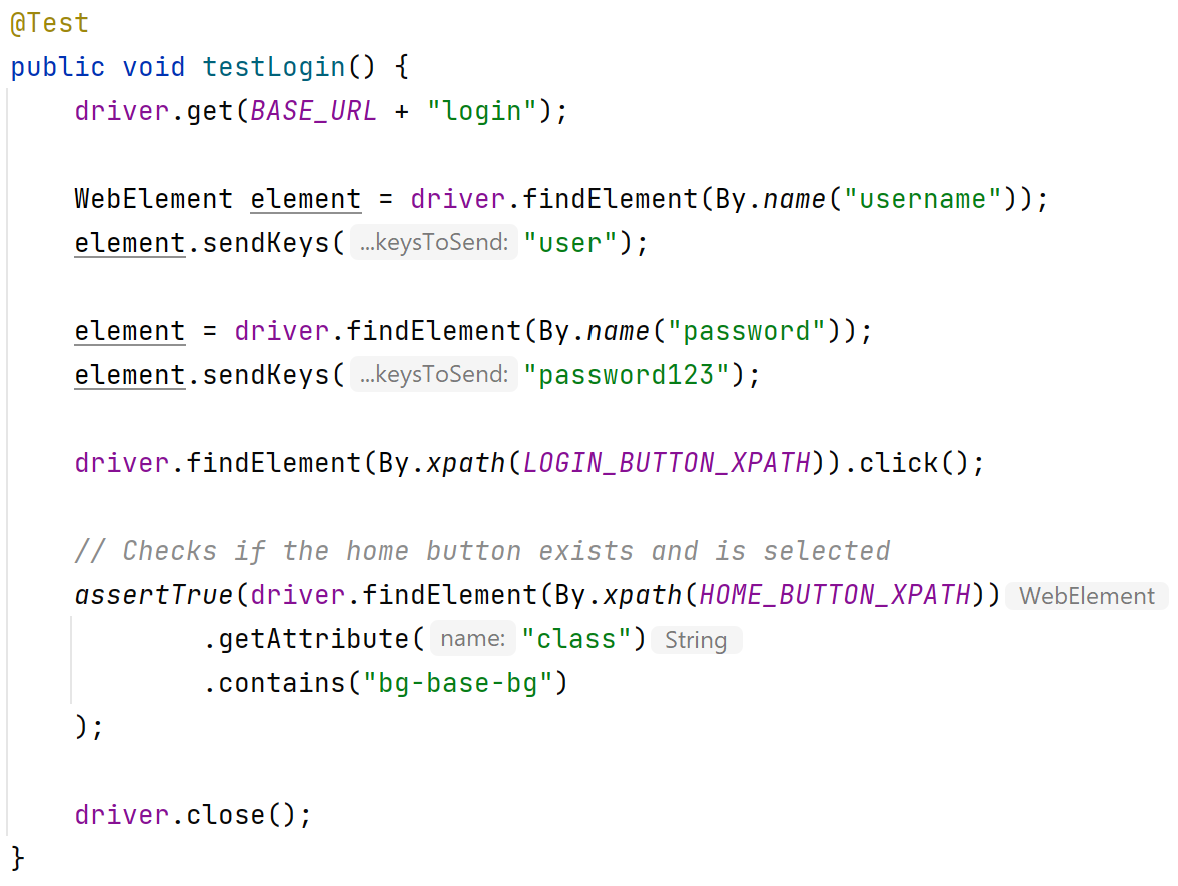
\includegraphics[scale=1]{slike/integration_test_login.png}
        		  \centering
        		\caption{Ispitni slučaj - prijava}
        	\end{figure}
                
                \begin{figure}[H]
        		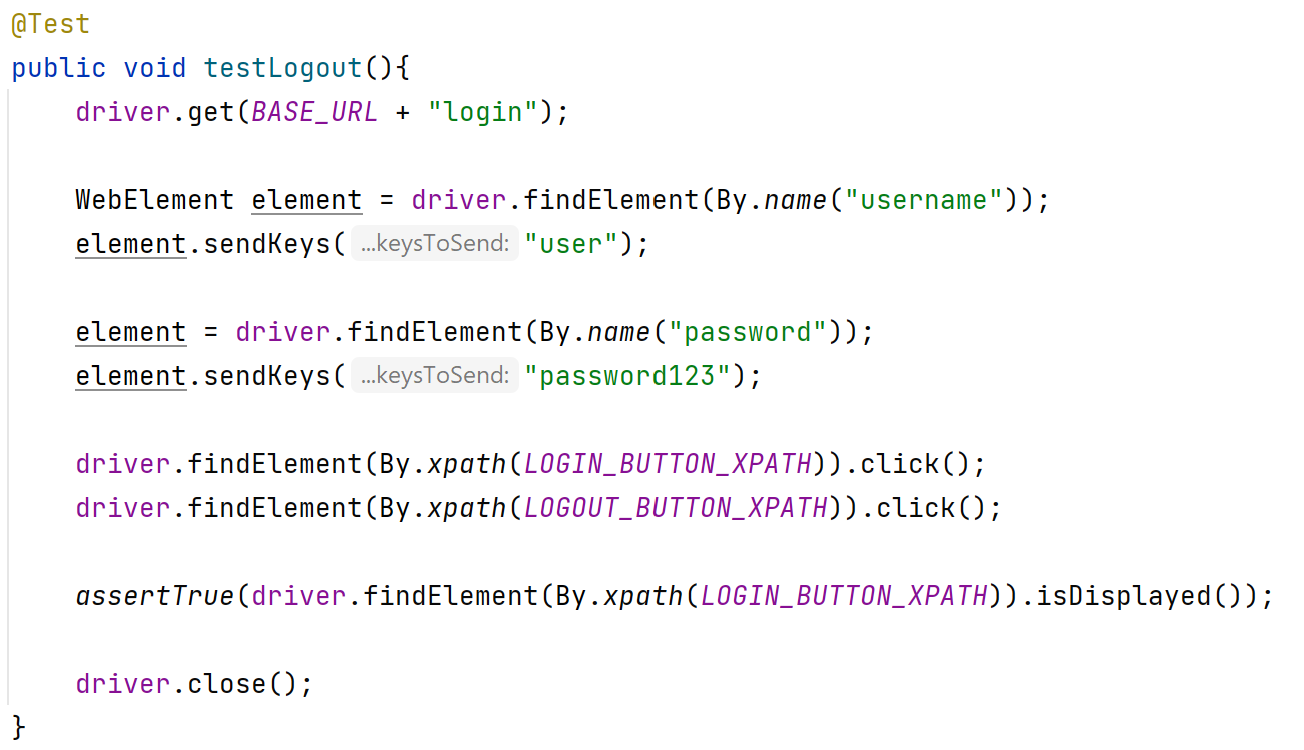
\includegraphics[scale=0.9]{slike/integration_test_logout.png} 
        		  \centering
        		\caption{Ispitni slučaj - odjava}
        	\end{figure}

                \begin{figure}[H]
        		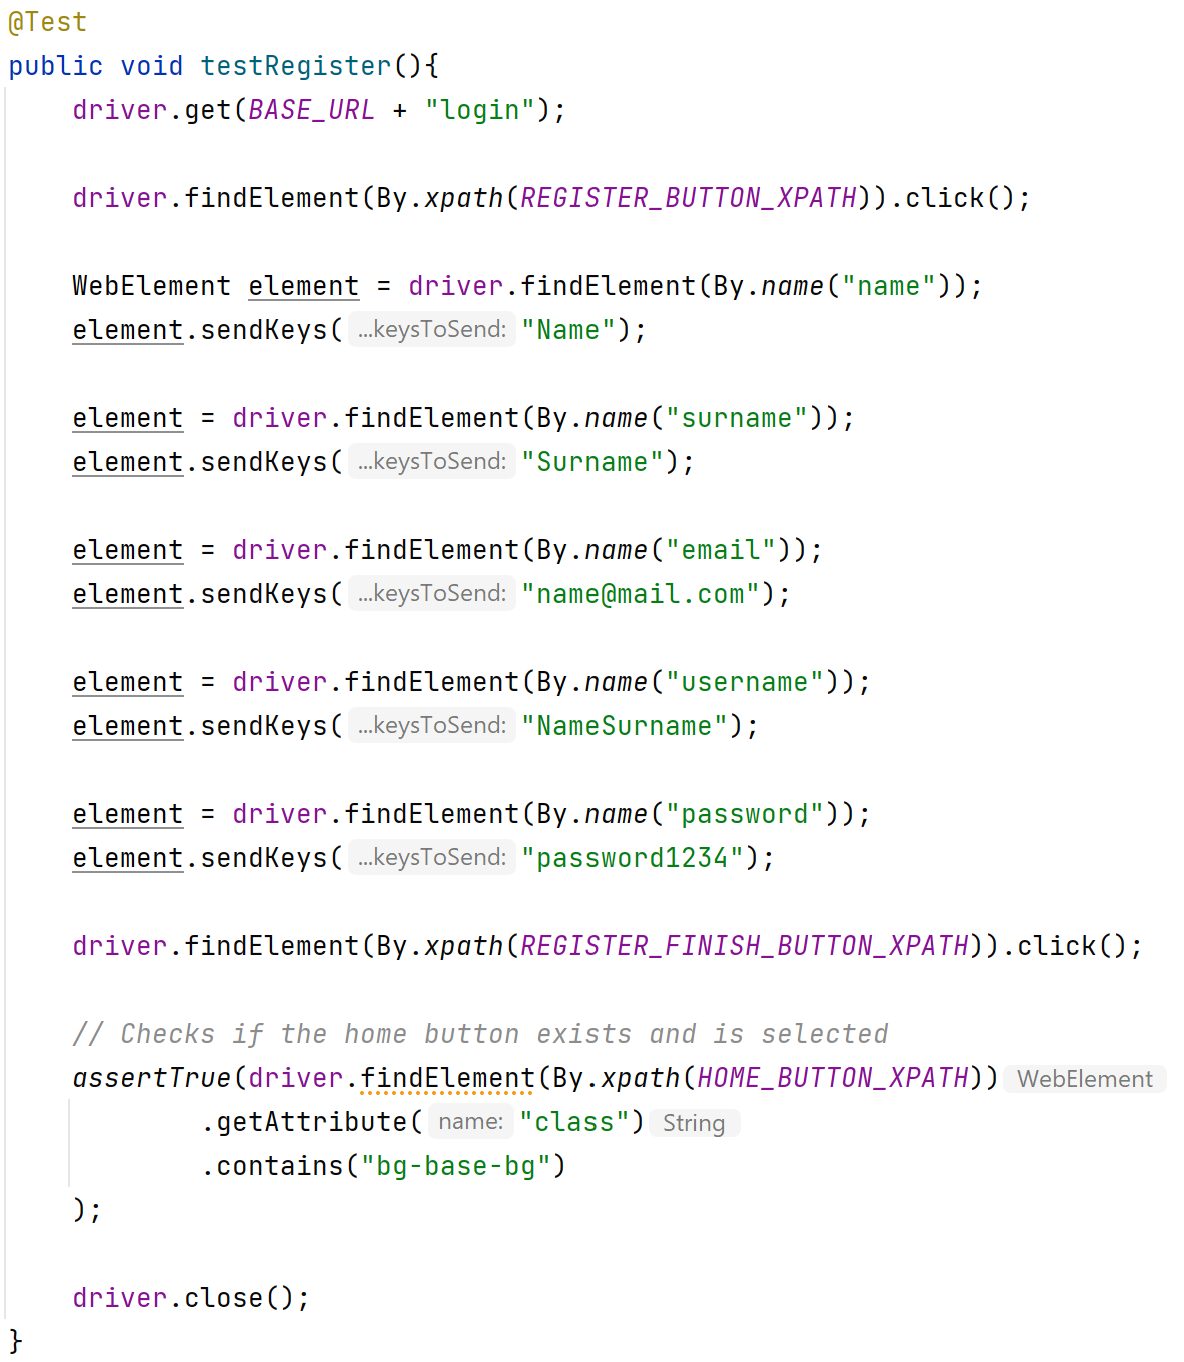
\includegraphics[scale=1]{slike/integration_test_register.png} 
        		  \centering
        		\caption{Ispitni slučaj - registracija}
        	\end{figure}

                \begin{figure}[H]
        		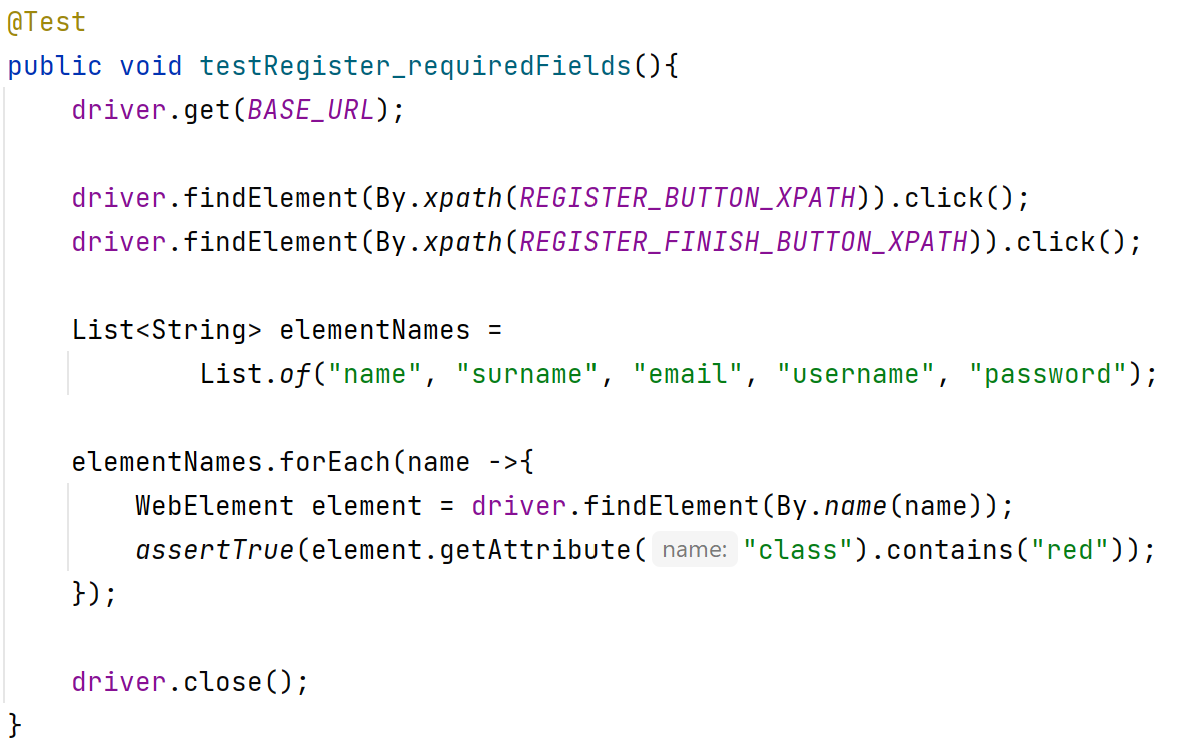
\includegraphics[scale=1]{slike/integration_test_register_required_fields.png} 
        		  \centering
        		\caption{Ispitni slučaj - validacija polja tijekom registracije}
        	\end{figure}
   
                \begin{figure}[H]
        		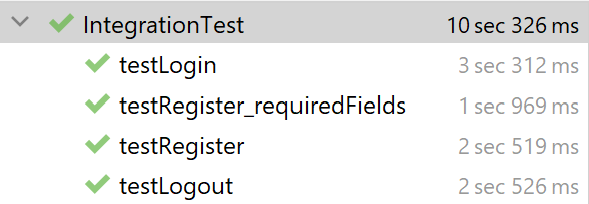
\includegraphics[scale=1]{slike/integration_test_results.png} 
        		  \centering
        		\caption{Rezultati ispitivanja sustava}
        	\end{figure}
		
			\eject 
		
		
		\section{Dijagram razmještaja}
			
			%\textbf{\textit{dio 2. revizije}}
			
			 %\textit{Potrebno je umetnuti \textbf{specifikacijski} dijagram razmještaja i opisati ga. Moguće je umjesto specifikacijskog dijagrama razmještaja umetnuti dijagram razmještaja instanci, pod uvjetom da taj dijagram bolje opisuje neki važniji dio sustava.}

            Dijagram razmještaja opisuje topologiju sklopovlja i programsku potporu koja se koristi u implementaciji. Korisnici koriste web preglednik kako bi pristupili web aplikaciji. Trenutna implementacija koristi dva različita poslužitelja, Heroku kao \textit{backend} poslužitelja i Render kao \textit{frontend} poslužitelja i poslužitelja baze podataka.
			\begin{figure}[H]
        		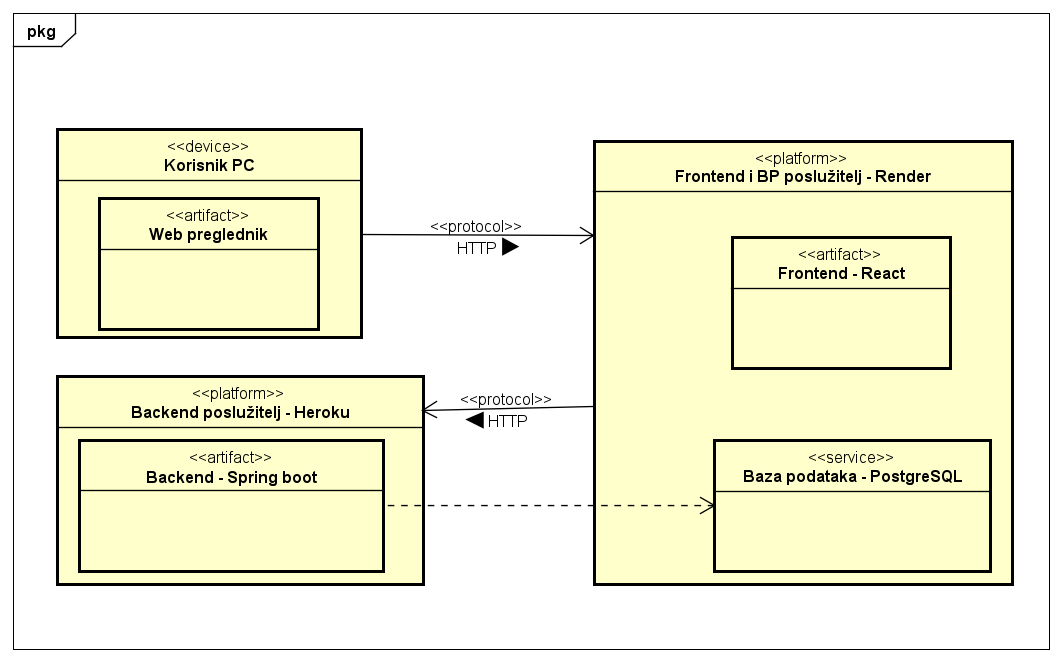
\includegraphics[scale=0.55]{slike/Dijagram razmjeÅ¡taja.png} %veličina slike u odnosu na originalnu datoteku i pozicija slike
        		  \centering
        		\caption{Dijagram razmještaja}

        	\end{figure}
			\eject 
		
		\section{Upute za puštanje u pogon}
		
			%&\textbf{\textit{dio 2. revizije}}\\
		
			% \textit{U ovom poglavlju potrebno je dati upute za puštanje u pogon (engl. deployment) ostvarene aplikacije. Na primjer, za web aplikacije, opisati postupak kojim se od izvornog kôda dolazi do potpuno postavljene baze podataka i poslužitelja koji odgovara na upite korisnika. Za mobilnu aplikaciju, postupak kojim se aplikacija izgradi, te postavi na neku od trgovina. Za stolnu (engl. desktop) aplikaciju, postupak kojim se aplikacija instalira na računalo. Ako mobilne i stolne aplikacije komuniciraju s poslužiteljem i/ili bazom podataka, opisati i postupak njihovog postavljanja. Pri izradi uputa preporučuje se \textbf{naglasiti korake instalacije uporabom natuknica} te koristiti što je više moguće \textbf{slike ekrana} (engl. screenshots) kako bi upute bile jasne i jednostavne za slijediti.}
			
			
			 %\textit{Dovršenu aplikaciju potrebno je pokrenuti na javno dostupnom poslužitelju. Studentima se preporučuje korištenje neke od sljedećih besplatnih usluga: \href{https://aws.amazon.com/}{Amazon AWS}, \href{https://azure.microsoft.com/en-us/}{Microsoft Azure} ili \href{https://www.heroku.com/}{Heroku}. Mobilne aplikacije trebaju biti objavljene na F-Droid, Google Play ili Amazon App trgovini.}

            \textbf{Instalacija poslužitelja baze podataka}
            \\
            Potrebno je preuzeti Docker Desktop aplikaciju. Za operacijski sustav Windows potrebno je instalirati i WSL2 podršku. Provodi se standardna instalacija s postavljanjem korisnika.
            \\
            \\
            \textbf{Pokretanje poslužitelja baze podataka}
            \\
    	Nakon instalacije potrebno je pokrenuti Docker kontejner preko `docker-compose.yaml` datoteke. Pozicionira se u direktorij gdje se datoteka nalazi te se pokreće korištenjem naredbe `docker-compose up`. U datoteci se nalazi potrebna konfiguracija za podizanje PostgreSQL baze podataka, sa postavljenim sučeljima i informacijama za spajanje.
            \\
            \\
            \textbf{Pokretanje poslužiteljske strane aplikacije}
            \\
            Potrebno je instalirati Gradle i Java programsku podršku. Nakon instalacije potrebno se pozicionirati u root direktorij aplikacije te pokrenuti naredbu `gradlew assemble`. Nakon što se aplikacija kompajlira, za pokretanje je potrebno upisati naredbu "`java -jar build/libs/[naziv\_izvršne\_datoteke].jar`.
            \\
            \\
            \textbf{Spajanje sa bazom podataka}
            \\
            Za stvaranje konekcije prema bazi podataka koristi se konfiguracija unutar aplikacije. Za aplikaciju je pri pokretanju potrebno definirati sve varijable okruženja potrebne za konfiguraciju, kao što su varijable za spajanje na bazu podataka. Primjer: `java -jar build/libs/app.jar -Dserver.port=8080 -DB\_URL=jdbc:postgresql://db.url -DB\_USERNAME=username -DB\_PASSWORD=password -DB\_SCHEMA=schema`.
            \\
            \eject
            \\
            \textbf{Pokretanje klijentske strane aplikacije}
            \\
            Za pokretanje klijentske strane potrebno je instalirati Node.js programsku podršku. Nakon instalacije potrebno se pozicionirati u root direktorij poslužiteljske aplikacije te izvršiti naredbu `npm run build`. Nakon izgradnje statičke stranice sa svim potrebnim resursima, poslužiteljska aplikacija za serviranje tih resursa pokreće se naredbom `npm start`.
            \\
            \\
            \textbf{Spajanje klijentske i poslužiteljske strane aplikacije}
            \\
            Isto kao i kod spajanja na bazu podataka, klijentska aplikacija ima konfiguriranog posrednika (eng. "proxy") pomoću kojeg se spaja prema poslužiteljskoj aplikaciji. Potrebno je dodati varijable okruženja pri pokretanju aplikacije. Primjer: `PORT=3000 APP\_BASE\_URL=https://url.do.posluzitelja node app.js
            
			
			\eject 
